\section{Auswertung}
\label{sec:Auswertung}

Zur Analyse der Kennlinien der Hochvakkumdiode werden für verschiedene Heizstromstärken
$I_\text{H,1}$ bis $I_\text{H,5}$ von $\SI{2.1}{\ampere}$, $\SI{2.2}{\ampere}$, $\SI{2.3}{\ampere}$, $\SI{2.4}{\ampere}$
und $\SI{2.5}{\ampere}$ die Diodenströme $I_1$ bis $I_5$ abhängig von der Spannung $U$ gemessen.
Die zugehörigen Messwerte sind in Tabelle \ref{tab:mess1} aufgelistet.

\begin{table}
  \footnotesize
  \centering
  \caption{Messwerte der Diodenströme $I_1$ bis $I_5$}
  \label{tab:mess1}
  \sisetup{table-format=2.1}
  \begin{tabular}{c c c c c c}
  \toprule
  $ U \,/\, \si{\volt} $ & $I_1 \,/\, \si{\milli\ampere}$ & $I_2 \,/\, \si{\milli\ampere}$
  & $I_3 \,/\, \si{\milli\ampere}$ & $I_4 \,/\, \si{\milli\ampere}$ 
  & $I_5 \,/\, \si{\milli\ampere}$ \\
  \midrule 
  0 & 0,000 & 0,000 & 0,000 & 0,000 & 0,000 \\
  5 & 0,007 & 0,011 & 0,014 & 0,014 & 0,014 \\
 10 & 0,019 & 0,031 & 0,034 & 0,038 & 0,033 \\
 15 & 0,033 & 0,054 & 0,058 & 0,059 & 0,053 \\
 20 & 0,050 & 0,080 & 0,085 & 0,087 & 0,079 \\
 25 & 0,070 & 0,105 & 0,114 & 0,116 & 0,108 \\
 30 & 0,093 & 0,131 & 0,146 & 0,148 & 0,144 \\
 35 & 0,114 & 0,163 & 0,179 & 0,182 & 0,178 \\
 40 & 0,136 & 0,190 & 0,211 & 0,215 & 0,216 \\
 45 & 0,155 & 0,224 & 0,245 & 0,254 & 0,257 \\
 50 & 0,176 & 0,252 & 0,275 & 0,297 & 0,302 \\
 55 & 0,195 & 0,284 & 0,317 & 0,342 & 0,349 \\
 60 & 0,213 & 0,312 & 0,352 & 0,362 & 0,391 \\
 65 & 0,228 & 0,348 & 0,392 & 0,425 & 0,454 \\
 70 & 0,241 & 0,370 & 0,427 & 0,475 & 0,510 \\
 75 & 0,250 & 0,402 & 0,483 & 0,532 & 0,563 \\
 80 & 0,258 & 0,437 & 0,530 & 0,592 & 0,623 \\
 85 & 0,266 & 0,470 & 0,572 & 0,649 & 0,681 \\
 90 & 0,272 & 0,501 & 0,622 & 0,709 & 0,741 \\
 95 & 0,278 & 0,530 & 0,663 & 0,763 & 0,805 \\
100 & 0,283 & 0,552 & 0,704 & 0,814 & 0,857 \\
105 & 0,288 & 0,577 & 0,751 & 0,878 & 0,922 \\
110 & 0,293 & 0,602 & 0,797 & 0,935 & 0,988 \\
115 & 0,297 & 0,623 & 0,844 & 0,961 & 1,047 \\
120 & 0,299 & 0,643 & 0,879 & 1,011 & 1,109 \\
125 & 0,301 & 0,659 & 0,922 & 1,076 & 1,160 \\
130 & 0,303 & 0,672 & 0,930 & 1,149 & 1,262 \\
135 &   -   & 0,681 & 0,965 & 1,225 & 1,354 \\
140 & 0,304 & 0,693 & 1,007 & 1,278 & 1,425 \\
145 &   -   & 0,702 & 1,044 & 1,336 & 1,496 \\
150 & 0,305 & 0,711 & 1,080 & 1,382 & 1,563 \\
155 &   -   & 0,716 & 1,112 & 1,437 & 1,626 \\
160 &   -   & 0,721 & 1,142 & 1,479 & 1,692 \\
165 &   -   & 0,713 & 1,169 & 1,527 & 1,768 \\
170 &   -   & 0,716 & 1,192 & 1,579 & 1,825 \\
175 &   -   &   -   &   -   & 1,628 & 1,895 \\
180 &   -   & 0,723 & 1,231 & 1,681 & 1,959 \\
185 &   -   &   -   &   -   & 1,721 & 2,030 \\
190 &   -   & 0,728 & 1,266 & 1,772 & 2,090 \\
195 &   -   &   -   &   -   & 1,820 & 2,160 \\
200 & 0,315 & 0,733 & 1,299 & 1,866 & 2,230 \\
205 &   -   &   -   &   -   & 1,914 & 2,310 \\
210 &   -   &   -   & 1,328 & 1,957 & 2,370 \\
215 &   -   &   -   &   -   & 1,999 & 2,450 \\
220 &   -   & 0,742 & 1,350 & 2,050 & 2,510 \\
225 &   -   &   -   &   -   & 2,090 & 2,580 \\
230 &   -   &   -   & 1,369 & 2,120 & 2,650 \\
235 &   -   &   -   &   -   & 2,170 & 2,720 \\
240 &   -   & 0,749 & 1,382 & 2,210 & 2,790 \\
245 &   -   &   -   &   -   & 2,240 & 2,850 \\
250 & 0,322 & 0,752 & 1,395 & 2,280 & 2,930 \\
  \bottomrule
  \end{tabular}
  \end{table}

In Abbildung \ref{fig:plot1} sind die Kennlinen der Hochvakkumdiode, d.h. die Messwerte der Diodenströme 
$I_\text{k}$ gegen die Spannung $U$ aufgetragen. 

\begin{figure} [H]
  \centering
  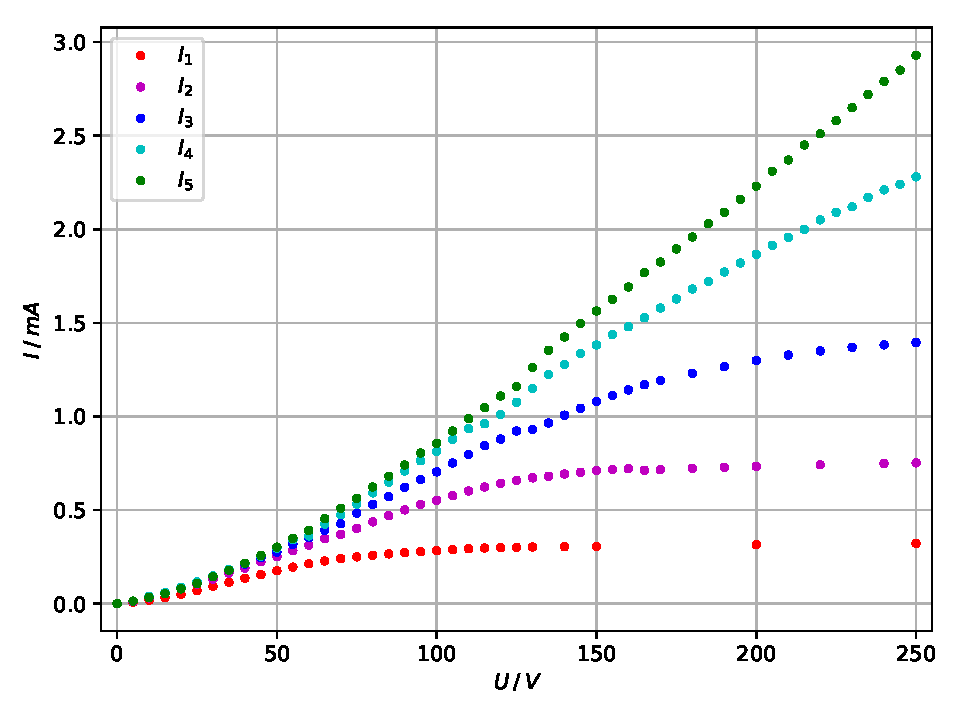
\includegraphics{content/plot1.pdf}
  \caption{Kennlinen der Hochvakkumdiode für verschiedene Heizstromstärken $I_\text{H,k}$}
  \label{fig:plot1}
\end{figure}

Aus der Abbildung \ref{fig:plot1} sind somit folgende Sättigungsstromstärken $I_\text{S,k}$ abblesbar:

\begin{align*}
  I_\text{S,1} &= \SI{0.3 }{\milli\ampere} \\
  I_\text{S,2} &= \SI{0.75}{\milli\ampere} \\
  I_\text{S,3} &= \SI{1.4}{\milli\ampere}
\end{align*}

Die Sättigungsstromstärke $I_\text{S,4}$ lässt sich aus den Messwerten etwa als $\SI{2.5}{\milli\ampere}$
erahnen, während $I_\text{S,5}$ gar nicht ablesbar ist.

\subsection{Untersuchung des Raumladungs- und des Anlaufstromgebietes für $I_\text{H,5}$}

Für die Heizstromstärke $I_\text{H,5} = \SI{2.5}{\ampere}$ wird die Kennlinie genauer untersucht.
Für das Raumladungsgebiet von etwa $\SI{0}{\volt}$ bis $\SI{25}{\volt}$ sind die Messwerte
in Abbildung \ref{fig:plot2} doppellogarithmisch aufgetragen.

\begin{figure} [H]
  \centering
  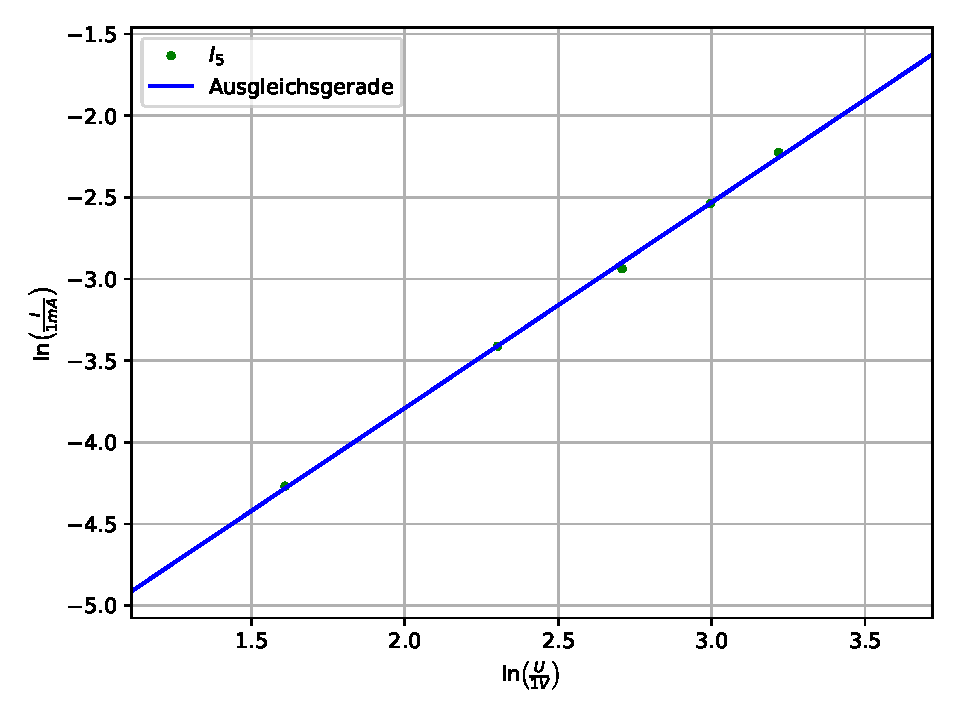
\includegraphics{content/plot2.pdf}
  \caption{Kennline der Hochvakkumdiode im Raumladungsgebiet mit der Heizstromstärke $I_\text{H,5}$}
  \label{fig:plot2}
\end{figure}

Aus der mit python bestimmten linearen Regression der Form 

\begin{equation*}
    \text{ln} \left(\frac{I}{\SI{1}{\milli\ampere}} \right) 
    = a \cdot \text{ln} \left(\frac{U}{\SI{1}{\volt}} \right) + b
\end{equation*}

ergeben sich die Regressionsparameter 

\begin{align*}
    a &= 1,260  \pm 0,040 \\
    b &= -6,310 \pm 0,105 \; .
\end{align*}

Somit entspricht der Exponent der Strom-Spannungs-Beziehung $a = 1,260  \pm 0,040$.\\

Für die Untersuchung des Anlaufstromgebietes wird der Diodenstrom für die Spannung $U$ im 
Intervall $\SI{0}{\volt}$ bis $\SI{1}{\volt}$ gemessen. 

Da für die Messung ein Nanoamperemeter mit Widerstand $R = \SI{1}{\mega\ohm}$ eingesetzt wird,
müssen die gemessenen Spannungswerte zu

\begin{equation*}
    U_\text{k} = U + I \cdot R
\end{equation*}

korrigiert werden.
Die (korrigierten) Messwerte sind in 
Tabelle \ref{tab:mess2} aufgelistet und werden in Abbildung \ref{fig:plot3}
einfachlogarithmisch gegeneinander aufgetragen.

\begin{table}
  \centering
  \caption{Messwerte des Diodenstroms im Anlaufstromgebiet}
  \label{tab:mess2}
  \sisetup{table-format=2.1}
  \begin{tabular}{c c c}
  \toprule
  $ U \,/\, \si{\volt} $ & $ U_\text{k} \,/\, \si{\volt} $ & $I_5 \,/\, \si{\nano\ampere}$\\
  \midrule 
  0,000 & 0,012 & 12,00 \\
  0,050 & 0,059 &  8,75 \\
  0,100 & 0,107 &  6,50 \\
  0,150 & 0,155 &  5,00 \\
  0,200 & 0,204 &  3,75 \\
  0,250 & 0,253 &  3,00 \\
  0,300 & 0,302 &  2,40 \\
  0,350 & 0,352 &  1,80 \\
  0,400 & 0,401 &  1,40 \\
  0,450 & 0,451 &  1,10 \\
  0,500 & 0,501 &  0,80 \\
  0,550 & 0,551 &  0,60 \\
  0,600 & 0,601 &  0,50 \\
  0,650 & 0,650 &  0,42 \\
  0,700 & 0,700 &  0,35 \\
  0,750 & 0,750 &  0,28 \\
  0,800 & 0,800 &  0,20 \\
  0,850 & 0,850 &  0,18 \\
  0,900 & 0,900 &  0,15 \\
  0,950 & 0,950 &  0,10 \\
  \bottomrule
  \end{tabular}
  \end{table}

  \begin{figure} [H]
    \centering
    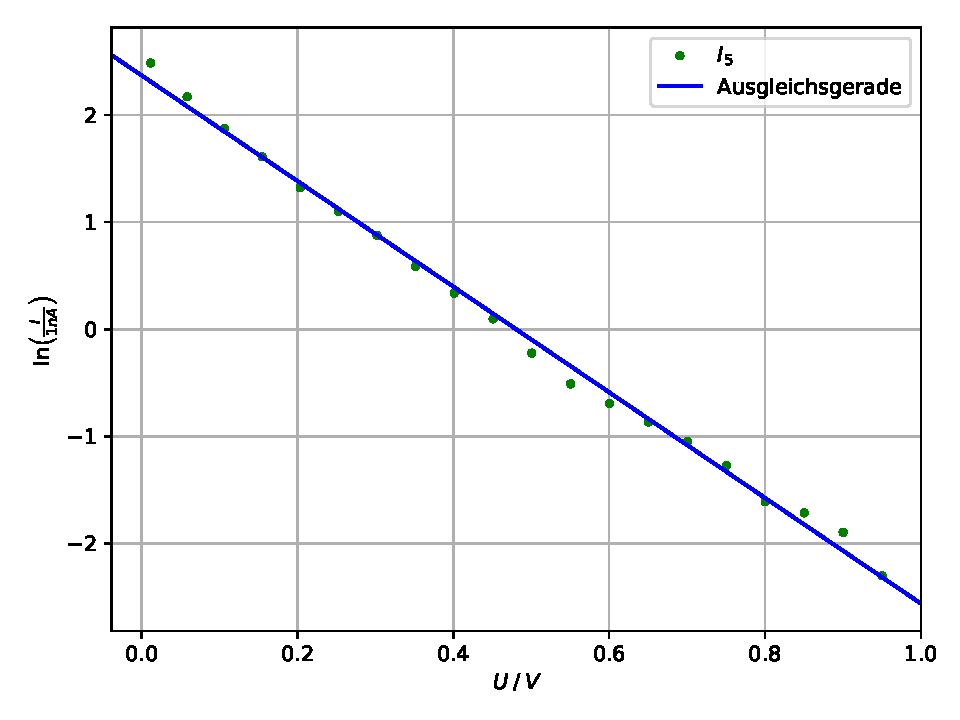
\includegraphics{content/plot3.pdf}
    \caption{Kennline der Hochvakkumdiode im Anlaufstromgebiet mit der Heizstromstärke $I_\text{H,5}$}
    \label{fig:plot3}
  \end{figure}

Aus der mit python bestimmten linearen Regression der Form 

\begin{equation*}
    \text{ln} \left(\frac{I}{\SI{1}{\milli\ampere}} \right) 
    = a \cdot U + b
\end{equation*}

ergeben sich die Regressionsparameter 

\begin{align*}
    a &= \SI{-4.888 +- 0.069}{\per\volt}\\
    b &= 2,337 \pm 0,039 \; .
\end{align*}

Im Vergleich mit der Gleichung \eqref{eqn:exponent} ergibt sich die Beziehung

\begin{equation*}
      a = - \frac{e}{kT} \; ,
\end{equation*}

durch welche sich nach Umstellung die Kathodentemperatur zu

\begin{equation}
      T = - \frac{e}{k \cdot a} = \SI{2490 +- 40}{\degree\kelvin}
\end{equation}

ergibt. \\

Die Kathodentemperatur $T$ lässt sich auch nach der Gleichung

\begin{equation}
    T = \left( \frac{I_\text{H} U_\text{H} - N_\text{WL}}{f \eta \sigma} \right)^{\frac{1}{4}}
    \label{eqn:temp}
\end{equation}

bestimmen. Die abgeschätzte Wärmeleitung  beträgt $N_\text{WL} = \SI{1}{\watt}$.
Weitere Größen sind die Stefan-Boltzmannsche Strahlungskonstante 
$\sigma = \num{5.7e-12}\frac{\text{W}}{\text{cm}^2\text{K}^4}$, die emmitierende Kathodenfläche
$\SI{0.35}{\centi\meter\squared}$ und der Oberflächenemisionsgrad $\eta = \num{0.28}$.

Des Weiteren werden die Austrittsarbeiten 

\begin{equation}
    e \phi = -k T \: \text{ln} \left( \frac{I_\text{S} h^3}{f 4 \pi e m k^2 T^2} \right)
    \label{eqn:ephi}
\end{equation}

berechnet.



Die gemessenen Sättigungsstromstärken, Heizstromstärken und -spannungen, sowie die nach 
\eqref{eqn:temp} und \eqref{eqn:ephi} berechneten Kathodentemperaturen $T$ und 
Austrittsarbeiten $e\phi$ befinden sich in Tabelle \ref{tab:mess3}.

\begin{table}
  \centering
  \caption{Messwerte der Sättigungsstromstärken, Heizstromstärken und -spannungen, sowie die daraus errechneten
          Kathodentemperaturen $T$ und Austrittsarbeiten $e\phi$}
  \label{tab:mess3}
  \sisetup{table-format=2.1}
  \begin{tabular}{c c c c c}
  \toprule
  $I_\text{H} \,/\, \si{\ampere} $ & $U_\text{H} \,/\, \si{\volt}$ & $T \,/\, \si{\kelvin}$
  & $I_\text{S} \,/\, \si{\milli\ampere} $ & $e\phi \,/\, \si{\eV} $\\
  \midrule 
    2,1 & 4,5 & 1972,15 & 0,30 & 5,81 \\
    2,2 & 4,8 & 2033,95 & 0,75 & 5,85 \\
    2,3 & 5,2 & 2104,64 & 1,40 & 5,96 \\
    2,4 & 5,5 & 2161,80 & 2,50 & 6,02 \\
    2,5 & 5,8 & 2217,22 &  -   &  -   \\
  \bottomrule
  \end{tabular}
  \end{table}

Der Mittelwert der Austrittsarbeiten beträgt 

\begin{equation*}
    \overline{e\phi} = \SI{5.91 +- 0.05}{\eV} \; .
\end{equation*}

